\documentclass[11pt]{article}
\usepackage[margin=1in]{geometry}
\usepackage{amsmath,amssymb,booktabs,graphicx,hyperref,xcolor,multirow,siunitx,caption,float}
\usepackage[numbers,sort&compress]{natbib}
% auto-generated by scripts/final_report.py -- do not edit
\newcommand{\TErmAurocAll}{0.733}
\newcommand{\TErmAurocDev}{0.758}
\newcommand{\TErmAurocConf}{0.707}
\newcommand{\TErmWorstFold}{0.565}
\newcommand{\TErmBalAcc}{0.634}
\newcommand{\TErmEce}{0.157}
\newcommand{\TErmDiffVsErm}{0.000}
\newcommand{\TGroupdroAurocAll}{0.748}
\newcommand{\TGroupdroAurocDev}{0.761}
\newcommand{\TGroupdroAurocConf}{0.735}
\newcommand{\TGroupdroWorstFold}{0.657}
\newcommand{\TGroupdroBalAcc}{0.689}
\newcommand{\TGroupdroEce}{0.144}
\newcommand{\TGroupdroDiffVsErm}{0.015}
\newcommand{\TGroupdroLo}{\ensuremath{-}0.015}
\newcommand{\TGroupdroHi}{0.055}
\newcommand{\TGroupdroFoldsBetter}{4}
\newcommand{\TDannAurocAll}{0.727}
\newcommand{\TDannAurocDev}{0.752}
\newcommand{\TDannAurocConf}{0.702}
\newcommand{\TDannWorstFold}{0.645}
\newcommand{\TDannBalAcc}{0.599}
\newcommand{\TDannEce}{0.166}
\newcommand{\TDannDiffVsErm}{\ensuremath{-}0.006}
\newcommand{\TDannLo}{\ensuremath{-}0.049}
\newcommand{\TDannHi}{0.035}
\newcommand{\TDannFoldsBetter}{4}
\newcommand{\TGenericAugAurocAll}{0.732}
\newcommand{\TGenericAugAurocDev}{0.748}
\newcommand{\TGenericAugAurocConf}{0.716}
\newcommand{\TGenericAugWorstFold}{0.619}
\newcommand{\TGenericAugBalAcc}{0.663}
\newcommand{\TGenericAugEce}{0.150}
\newcommand{\TGenericAugDiffVsErm}{\ensuremath{-}0.001}
\newcommand{\TGenericAugLo}{\ensuremath{-}0.029}
\newcommand{\TGenericAugHi}{0.032}
\newcommand{\TGenericAugFoldsBetter}{3}
\newcommand{\TSiteProfileAugAurocAll}{0.726}
\newcommand{\TSiteProfileAugAurocDev}{0.757}
\newcommand{\TSiteProfileAugAurocConf}{0.694}
\newcommand{\TSiteProfileAugWorstFold}{0.641}
\newcommand{\TSiteProfileAugBalAcc}{0.618}
\newcommand{\TSiteProfileAugEce}{0.174}
\newcommand{\TSiteProfileAugDiffVsErm}{\ensuremath{-}0.007}
\newcommand{\TSiteProfileAugLo}{\ensuremath{-}0.060}
\newcommand{\TSiteProfileAugHi}{0.038}
\newcommand{\TSiteProfileAugFoldsBetter}{6}
\newcommand{\TProfileAdversaryPaiAurocAll}{0.730}
\newcommand{\TProfileAdversaryPaiAurocDev}{0.753}
\newcommand{\TProfileAdversaryPaiAurocConf}{0.708}
\newcommand{\TProfileAdversaryPaiWorstFold}{0.551}
\newcommand{\TProfileAdversaryPaiBalAcc}{0.615}
\newcommand{\TProfileAdversaryPaiEce}{0.154}
\newcommand{\TProfileAdversaryPaiDiffVsErm}{\ensuremath{-}0.002}
\newcommand{\TProfileAdversaryPaiLo}{\ensuremath{-}0.020}
\newcommand{\TProfileAdversaryPaiHi}{0.014}
\newcommand{\TProfileAdversaryPaiFoldsBetter}{4}
\newcommand{\TSidlCcAurocAll}{0.711}
\newcommand{\TSidlCcAurocDev}{0.722}
\newcommand{\TSidlCcAurocConf}{0.699}
\newcommand{\TSidlCcWorstFold}{0.635}
\newcommand{\TSidlCcBalAcc}{0.612}
\newcommand{\TSidlCcEce}{0.178}
\newcommand{\TSidlCcDiffVsErm}{\ensuremath{-}0.022}
\newcommand{\TSidlCcLo}{\ensuremath{-}0.069}
\newcommand{\TSidlCcHi}{0.030}
\newcommand{\TSidlCcFoldsBetter}{3}
\newcommand{\TSidlPhysAurocAll}{0.744}
\newcommand{\TSidlPhysAurocDev}{0.756}
\newcommand{\TSidlPhysAurocConf}{0.732}
\newcommand{\TSidlPhysWorstFold}{0.650}
\newcommand{\TSidlPhysBalAcc}{0.656}
\newcommand{\TSidlPhysEce}{0.192}
\newcommand{\TSidlPhysDiffVsErm}{0.011}
\newcommand{\TSidlPhysLo}{\ensuremath{-}0.016}
\newcommand{\TSidlPhysHi}{0.050}
\newcommand{\TSidlPhysFoldsBetter}{3}
\newcommand{\TSidlFullAurocAll}{0.701}
\newcommand{\TSidlFullAurocDev}{0.738}
\newcommand{\TSidlFullAurocConf}{0.665}
\newcommand{\TSidlFullWorstFold}{0.415}
\newcommand{\TSidlFullBalAcc}{0.590}
\newcommand{\TSidlFullEce}{0.175}
\newcommand{\TSidlFullDiffVsErm}{\ensuremath{-}0.031}
\newcommand{\TSidlFullLo}{\ensuremath{-}0.085}
\newcommand{\TSidlFullHi}{0.016}
\newcommand{\TSidlFullFoldsBetter}{3}
\newcommand{\CLsoCvplusCovMean}{0.942}
\newcommand{\CLsoCvplusCovMin}{0.867}
\newcommand{\CLsoCvplusSize}{1.747}
\newcommand{\CLsoCvplusNUnder}{0}
\newcommand{\CLsoCvplusN}{8}
\newcommand{\CLsoCvplusCovCalibErr}{0.041}
\newcommand{\CLsoCvplusFracUnder}{0.069}
\newcommand{\CLsoCvplusSizeAtCov}{1.602}
\newcommand{\CLsoCvplusBalCovMean}{0.926}
\newcommand{\CLsoCvplusBalCovMin}{0.792}
\newcommand{\CLsoCvplusBalSize}{1.687}
\newcommand{\CLsoCvplusBalNUnder}{1}
\newcommand{\CLsoCvplusBalN}{8}
\newcommand{\CLsoCvplusBalCovCalibErr}{0.020}
\newcommand{\CLsoCvplusBalFracUnder}{0.153}
\newcommand{\CLsoCvplusBalSizeAtCov}{1.603}
\newcommand{\CLsoSplitCovMean}{0.905}
\newcommand{\CLsoSplitCovMin}{0.732}
\newcommand{\CLsoSplitSize}{1.590}
\newcommand{\CLsoSplitNUnder}{1}
\newcommand{\CLsoSplitN}{8}
\newcommand{\CLsoSplitCovCalibErr}{0.011}
\newcommand{\CLsoSplitFracUnder}{0.208}
\newcommand{\CLsoSplitSizeAtCov}{1.574}
\newcommand{\CLsoSplitBalCovMean}{0.886}
\newcommand{\CLsoSplitBalCovMin}{0.711}
\newcommand{\CLsoSplitBalSize}{1.540}
\newcommand{\CLsoSplitBalNUnder}{1}
\newcommand{\CLsoSplitBalN}{8}
\newcommand{\CLsoSplitBalCovCalibErr}{0.009}
\newcommand{\CLsoSplitBalFracUnder}{0.236}
\newcommand{\CLsoSplitBalSizeAtCov}{1.578}
\newcommand{\CLsoWorstCovMean}{0.960}
\newcommand{\CLsoWorstCovMin}{0.832}
\newcommand{\CLsoWorstSize}{1.807}
\newcommand{\CLsoWorstNUnder}{1}
\newcommand{\CLsoWorstN}{8}
\newcommand{\CLsoWorstCovCalibErr}{0.083}
\newcommand{\CLsoWorstFracUnder}{0.028}
\newcommand{\CLsoWorstSizeAtCov}{1.588}
\newcommand{\CPooledCovMean}{0.836}
\newcommand{\CPooledCovMin}{0.743}
\newcommand{\CPooledSize}{1.389}
\newcommand{\CPooledNUnder}{4}
\newcommand{\CPooledN}{8}
\newcommand{\CPooledCovCalibErr}{0.048}
\newcommand{\CPooledFracUnder}{0.389}
\newcommand{\CPooledSizeAtCov}{1.582}
\newcommand{\CSiteBalancedCovMean}{0.840}
\newcommand{\CSiteBalancedCovMin}{0.746}
\newcommand{\CSiteBalancedSize}{1.376}
\newcommand{\CSiteBalancedNUnder}{4}
\newcommand{\CSiteBalancedN}{8}
\newcommand{\CSiteBalancedCovCalibErr}{0.053}
\newcommand{\CSiteBalancedFracUnder}{0.472}
\newcommand{\CSiteBalancedSizeAtCov}{1.603}
\newcommand{\CWorstSiteCovMean}{0.904}
\newcommand{\CWorstSiteCovMin}{0.751}
\newcommand{\CWorstSiteSize}{1.597}
\newcommand{\CWorstSiteNUnder}{2}
\newcommand{\CWorstSiteN}{8}
\newcommand{\CWorstSiteCovCalibErr}{0.009}
\newcommand{\CWorstSiteFracUnder}{0.236}
\newcommand{\CWorstSiteSizeAtCov}{1.582}
\newcommand{\OMeanSignedSeen}{0.118}
\newcommand{\OMeanSignedLso}{0.007}
\newcommand{\OMaeSeen}{0.130}
\newcommand{\OMaeLso}{0.070}
\newcommand{\ONUnits}{16}
\newcommand{\ORhoSeen}{\ensuremath{-}0.310}
\newcommand{\ORhoLso}{\ensuremath{-}0.048}
\newcommand{\ORhoGapCov}{\ensuremath{-}0.452}
\newcommand{\datasetTotal}{924}
\newcommand{\profLeakLogreg}{0.662}
\newcommand{\profLeakGbm}{0.588}
\newcommand{\priorSpreadSd}{0.274}
\newcommand{\siteAccProfile}{0.367}
\newcommand{\siteAccChance}{0.224}
\newcommand{\synthDiffErmP}{\ensuremath{-}0.000}
\newcommand{\synthDiffErmPLo}{\ensuremath{-}0.040}
\newcommand{\synthDiffErmPHi}{0.038}
\newcommand{\synthDiffDann}{\ensuremath{-}0.092}
\newcommand{\synthDiffDannLo}{\ensuremath{-}0.175}
\newcommand{\synthDiffDannHi}{\ensuremath{-}0.016}
\newcommand{\synthDiffCdann}{\ensuremath{-}0.077}
\newcommand{\synthDiffCdannLo}{\ensuremath{-}0.142}
\newcommand{\synthDiffCdannHi}{\ensuremath{-}0.019}
\newcommand{\synthDiffCdannP}{\ensuremath{-}0.047}
\newcommand{\synthDiffCdannPLo}{\ensuremath{-}0.092}
\newcommand{\synthDiffCdannPHi}{\ensuremath{-}0.013}
\newcommand{\rankCorrDevConf}{0.500}
\newcommand{\relErm}{0.438}
\newcommand{\relGroupdro}{0.423}
\newcommand{\relDann}{0.415}
\newcommand{\relGenericAug}{0.411}
\newcommand{\relSiteProfileAug}{0.396}
\newcommand{\relProfileAdversaryPai}{0.398}
\newcommand{\relSidlCc}{0.473}
\newcommand{\relSidlPhys}{0.422}
\newcommand{\relSidlFull}{0.514}
\newcommand{\ensAurocFull}{0.733}
\newcommand{\ensAurocEns}{0.748}
\newcommand{\ensDAuroc}{0.016}
\newcommand{\ensDAurocLo}{\ensuremath{-}0.008}
\newcommand{\ensDAurocHi}{0.049}
\newcommand{\ensDEce}{\ensuremath{-}0.003}
\newcommand{\ensFoldsBetter}{5}
\newcommand{\ensMembers}{9}

\captionsetup{font=small,labelfont=bf}
\newcommand{\erm}{ERM}
\newcommand{\method}{\textsc{SIDL}}

\title{Scanner-Invariant and Institution-Invariant Deep Learning for Reliable Medical Image Diagnosis Across Heterogeneous Clinical Environments\\[4pt]
\large A Leave-Site-Out Study of What Invariance Methods Do and Do Not Deliver, and How to Calibrate Prediction Sets for Unseen Sites}
\author{Anonymous Authors}
\date{}

\begin{document}
\maketitle

\begin{abstract}
Diagnostic image models often lose accuracy and calibration at hospitals that were not in the training data. We set out to build a scanner- and institution-invariant pipeline that combines class-conditional adversarial alignment, augmentation grounded in per-site acquisition profiles, and cross-site conformal prediction. We tested it with a leave-one-site-out protocol on an open multi-source chest-radiograph benchmark (924 images, 10 sources, COVID-19 versus other findings), with development folds for all design decisions and untouched confirmation folds for frozen configurations. Our main result is negative: over eight held-out sites and nine training methods, none significantly improved held-out AUROC over empirical risk minimization (\erm{}); every 95\% interval for the difference includes zero, the largest point gains are $+\TGroupdroDiffVsErm$ (GroupDRO) and $+\TSidlPhysDiffVsErm$ (one augmentation-plus-adversary variant), and strong augmentation or strong adversaries hurt. Three other observations held up. (i)~Five label-free acquisition statistics predict the diagnosis on unseen sites with AUROC $\profLeakLogreg$, so site-level acquisition signatures are a usable shortcut on this data. (ii)~Validation on sites seen in training overstates held-out AUROC by $\OMeanSignedSeen$ and standard split-conformal sets under-cover unseen sites (mean coverage $\CPooledCovMean$ against a $0.90$ target; $\CPooledNUnder$ of $\CPooledN$ sites more than five points short). Calibrating on scores from models that never saw the calibration site (a leave-site-out CV+ rule) left no site more than five points short, at the price of sets about $26\%$ larger; all calibration variants we tried lie on essentially one coverage--set-size curve, so they differ in operating point rather than efficiency. (iii)~A controlled simulation of acquisition shift did not reproduce the real under-coverage, so simulated shift is a poor stand-in for inter-hospital shift here. The benchmark is small, single-modality and trained from scratch on a CPU, and we make no claim about clinical COVID-19 detection. Code, frozen configurations and a script that regenerates every table and figure are released.
\end{abstract}

\section{Introduction}
Clinical deployment of diagnostic AI requires reliability across heterogeneous environments: scanner vendors, acquisition protocols, reconstruction kernels, patient populations and labeling practices. Models trained on pooled multi-institution data can learn shortcuts that correlate with the site~\cite{zech2018variable,degrave2021ai,geirhos2020shortcut}, which inflates in-distribution accuracy and can fail silently at a new site. A popular response is to make models \emph{invariant} to scanner and institution, using adversarial alignment, feature-statistics matching, harmonization or augmentation~\cite{ganin2016domain,sun2016deep,zhang2020generalizing,johnson2007adjusting}.

We began this project to build such a recipe and to publish the results. The recipe had three parts that each address a gap we believed existed: (1)~an adversary that aligns features \emph{within each class} across sites, so that differing disease prevalence between hospitals is not penalized~\cite{zhao2019learning}; (2)~augmentation that re-renders each image as if acquired at another \emph{observed} site, using acquisition statistics estimated label-free from the training images; and (3)~conformal prediction sets calibrated so that coverage degrades gracefully on an unseen site. We then ran what we considered the decisive experiment: a leave-one-site-out (LOSO) evaluation with a development/confirmation split and configurations frozen before the confirmation run.

\paragraph{What we found.} The accuracy-side recipe did not work on this data: no method, including ours, significantly beat \erm{}. What did hold up is a set of diagnostic and calibration results about \emph{why} and about \emph{how to report uncertainty honestly} for unseen sites. We report both, because negative results with a frozen protocol are informative to anyone choosing between these methods on small multi-site data.

\paragraph{Contributions.} We state these conservatively; we did not find these combinations in the work we reviewed (Section~\ref{sec:related}), but our search was targeted, not a systematic review.
\begin{enumerate}
  \item \textbf{A frozen leave-site-out protocol on open data.} Eight held-out sites, four used for every design decision and four untouched until a single frozen run, model selection on source sites only, and a hierarchical paired bootstrap that resamples sites and then test images (Section~\ref{sec:protocol}).
  \item \textbf{A systematic negative result for invariance recipes.} Nine methods, including three variants we implemented (class-conditional adversary with site-prior reweighting, site-profile augmentation, profile-adversarial invariance), none significantly better than \erm{}; a controlled label-shift sweep in which the ordering predicted by theory appears but adversaries never beat \erm{} (Sections~\ref{sec:task} and~\ref{sec:synth}).
  \item \textbf{Label-free acquisition diagnostics.} A profile-only leak score and a within-class shortcut-reliance score that need no site metadata beyond the site label (Section~\ref{sec:diag}). The idea that COVID-19 chest radiograph classifiers exploit dataset cues is established~\cite{maguolo2021critic,degrave2021ai,roberts2021common,tartaglione2020unveiling}; our diagnostic quantifies it with five numbers on held-out sites.
  \item \textbf{Evidence on calibrating prediction sets for unseen sites.} Seen-site validation is optimistic by about $0.12$ AUROC and this is accompanied by conformal under-coverage; a leave-site-out CV+ rule (CV+~\cite{barber2021predictive} with sites as folds) removes severe under-coverage; every calibration variant lies on one coverage--size curve; and simulated acquisition shift does not reproduce the real effect (Sections~\ref{sec:conf}--\ref{sec:realism}).
\end{enumerate}
We do not claim clinical COVID-19 detection performance. The benchmark is used as a shortcut-prone stress test of multi-site methodology.

\section{Related Work}\label{sec:related}
\paragraph{Shortcuts and shift in chest radiography.} Pneumonia and COVID-19 classifiers have been shown to depend on site, scanner and dataset artifacts~\cite{zech2018variable,pooch2020can}. For COVID-19 in particular, masking the central lung region barely changes accuracy on public collections~\cite{maguolo2021critic}, classifiers can select shortcuts over signal~\cite{degrave2021ai}, small-data pitfalls are catalogued~\cite{tartaglione2020unveiling}, and a large review found pervasive bias in the literature~\cite{roberts2021common}. Our diagnostics are in this tradition; they add a held-out-site, label-free measurement and use it to test invariance methods.

\paragraph{Domain generalization and invariance.} DANN~\cite{ganin2016domain}, conditional adversarial adaptation~\cite{long2018conditional}, CORAL~\cite{sun2016deep}, GroupDRO~\cite{sagawa2020distributionally}, IRM~\cite{arjovsky2019invariant} and MixStyle~\cite{zhou2021domain} target shift; DomainBed found that, under fair selection, no method reliably beats \erm{}~\cite{gulrajani2021in}, and WILDS reports similar difficulty on real shifts~\cite{koh2021wilds}. Exact feature invariance is provably limited when label priors differ between domains~\cite{zhao2019learning}, and adaptation methods address joint conditional and label shift when \emph{target} data are available~\cite{liu2021adversarial,lipton2018detecting}. We study the generalization setting without target data and find, consistently with DomainBed, no gain over \erm{}.

\paragraph{Acquisition-aware augmentation and harmonization.} BigAug stacks intensity, noise and blur transforms~\cite{zhang2020generalizing}; stain augmentation addresses histology~\cite{tellez2019quantifying}; ComBat removes batch effects in feature space~\cite{johnson2007adjusting}. Our site-profile augmentation estimates per-site statistics from the training images and translates between observed sites; it is a measurement-driven approximation and did not help here.

\paragraph{Conformal prediction under shift.} Split conformal prediction needs exchangeability~\cite{vovk2005algorithmic,angelopoulos2023gentle}; weighted and non-exchangeable variants handle known covariate shift or drift~\cite{tibshirani2019conformal,barber2023conformal}, label shift~\cite{podkopaev2021distribution} and multiple sources~\cite{liu2024multisource}. For unseen domains, worst-case calibration over source domains or divergence balls has been proposed~\cite{zou2024coverage}, and per-domain robust conformal calibration serves as a baseline in set-valued domain generalization~\cite{tsibulsky2025set}; pitfalls of conformal sets in medical imaging, including coverage failure under domain shift, are documented~\cite{mehrtens2025pitfalls}. Our worst-site mode is a variant of these ideas and we do not claim it as new. The CV+ rule comes from jackknife+~\cite{barber2021predictive}; we use sites as folds and measure the result on real held-out sites. We did not find a prior evaluation of exactly this site-fold CV+ on real multi-site medical images, but we did not search exhaustively.

\section{Setting and Methods}
\subsection{Problem setting}
Data come from $K$ source sites, $\mathcal{D}_k\sim P_k(X,Y)$, which differ in the acquisition process $P_k(X\mid Y)$ and in the prevalence $P_k(Y)$. A model is trained, selected and calibrated on source sites only and evaluated on a held-out site $K{+}1$. The label is binary (COVID-19 versus other finding). Let $z$ denote the encoder output, $c$ the task head and $s$ the site index.

\subsection{Training methods}
All methods share the same encoder, optimizer and budget (Section~\ref{sec:protocol}); each method differs only in the flags below.
\begin{itemize}
  \item \textbf{\erm{}} (cross-entropy), \textbf{GroupDRO} (sites as groups, step $0.01$)~\cite{sagawa2020distributionally}, \textbf{DANN} (unconditional site adversary through gradient reversal, weight $0.5$)~\cite{ganin2016domain}, \textbf{generic aug.} (intensity, gamma, noise, blur and bias-field transforms applied per sample).
  \item \textbf{Class-conditional adversary (cDANN).} One site discriminator $d_c$ per class, each behind a gradient-reversal layer, with each sample routed to the discriminator of its label, $\mathcal{L}_{\text{adv}}=\mathbb{E}\,\mathrm{CE}(d_y(\mathrm{GRL}_\lambda(z)),s)$. A discriminator that only sees one class cannot exploit between-site differences in $P_k(Y)$.
  \item \textbf{Class-conditional CORAL.} Pairwise mean and covariance matching of $z$ between sites, computed separately inside each class~\cite{sun2016deep}.
  \item \textbf{Site-prior reweighting.} Task-loss weights $w_{s,y}=\pi(y)/\pi_s(y)$ from the pooled prior $\pi$ and the site prior $\pi_s$ (smoothed, clipped).
  \item \textbf{Site-profile augmentation.} For each image we measure a profile $\theta(x)$ of mean, contrast, noise floor (MAD of a high-pass residual), sharpness (normalized gradient magnitude; a noise-compensated estimator, verified on the semi-synthetic data, was not used in the real-data runs) and low-frequency bias. For each training site $k$ we estimate mean $m_k$ and spread $S_k$ of $\theta$ with no labels. An image from site $s$ is translated toward a target site $t$ by applying only the \emph{relative} change (contrast/brightness matching, extra noise of variance $\max(\nu_t^2-\nu_s^2,0)$, blur or mild sharpening, a multiplicative low-frequency field) with strength $\alpha$ and probability $p$ per sample. This is a proxy, not a scanner simulator.
  \item \textbf{Profile-adversarial invariance (PAI).} A gradient-reversal head regresses the standardized \emph{measured} profile of the input from $z$ (optionally given the label), pushing $z$ to carry less measurable acquisition information.
  \item \textbf{SIDL variants.} \textsc{SIDL-cc}: generic aug.\ + cDANN + class-conditional CORAL + prior reweighting + consistency loss between clean and augmented views (weight $0.5$). \textsc{SIDL-phys}: site-profile aug.\ + unconditional DANN + pooled CORAL + consistency. \textsc{SIDL-full}: site-profile aug.\ + cDANN + class-conditional CORAL + prior reweighting + consistency.
\end{itemize}
Mild settings (augmentation probability $0.3$, strength $0.5$, adversary weight $0.1$ for SIDL and PAI, $0.5$ for DANN) were chosen on the development folds and frozen. Stronger settings are reported in the iteration log and hurt (Section~\ref{sec:task}).

\subsection{Label-free acquisition diagnostics}\label{sec:diagmethods}
\paragraph{Profile leak.} A logistic regression on the five-number profile is trained on source sites and scored on the held-out site; we report AUROC for the diagnosis. A value above $0.5$ means that acquisition statistics alone, with no anatomy, predict the label on unseen sites.
\paragraph{Shortcut reliance.} For a trained model we compute, within each class, the Spearman correlation between the model's held-out $P(\text{COVID-19})$ and the profile-only score above, then average over classes. Using within-class correlations means the label itself cannot explain a high value.

\subsection{Conformal calibration for unseen sites}\label{sec:confmethods}
We use the least-ambiguous score $r(x,y)=1-p_\theta(y\mid x)$~\cite{sadinle2019least} and prediction sets $\{y: r(x,y)\le\hat q\}$ for target miscoverage $\alpha$. We compare:
\begin{itemize}
  \item \textbf{Pooled, site-balanced, worst-site} (computed on the validation split of the seen source sites): the split-conformal quantile of all scores; a weighted quantile with equal total weight per site; the maximum per-site quantile over sites with at least $25$ images.
  \item \textbf{Leave-site-out (LSO) scores.} For every source site $k$ we train an inner model on the other source sites (with its own source-only validation split) and score \emph{all} images of site $k$ with it: $R_i=1-p_{-k(i)}(y_i\mid x_i)$. These scores mimic how a model behaves on a site it never saw.
  \item \textbf{LSO-split} applies the pooled quantile of the $R_i$ to the single deployed model; \textbf{LSO-worst} uses the maximum per-site quantile; \textbf{LSO-CV+} applies the CV+ rule with sites as folds: label $y$ is included for a test image $x$ iff
  $\#\{i: R_i < 1-p_{-k(i)}(y\mid x)\} < (1-\alpha)(n+1)$, where every inner model scores the test image; ``balanced'' variants weight each site equally.
\end{itemize}
CV+ has a finite-sample guarantee for exchangeable \emph{data points}~\cite{barber2021predictive}. Here the exchangeable units would have to be \emph{sites}, we have only $9$ source sites and we have no theorem; coverage is measured empirically on real held-out sites. We report coverage on the held-out site, mean set size, the number of held-out sites more than five points below target, the coverage-calibration error (mean $|\text{coverage}-(1-\alpha)|$ over $\alpha\in\{0.04,0.06,0.08,0.10,0.13,0.16,0.20,0.25,0.30\}$), the fraction of (site, $\alpha$) cells more than five points below target, and the set size interpolated at $90\%$ coverage along the fold-averaged coverage--size curve.

\section{Benchmark and Protocol}\label{sec:protocol}
\paragraph{Data.} We pooled three public GitHub collections of frontal chest radiographs: the COVID-19 image data collection~\cite{cohen2020covid}, the Actualmed collection~\cite{chung2020actualmed} and the Figure~1 collection~\cite{chung2020figure1}. The site is the reported institution or country in the metadata; sites with few images are merged into ``Other'' and images without location metadata form ``Unknown'', so these two groups are heterogeneous and are not single hospitals. The label is COVID-19 versus any other finding; lateral views and unlabeled rows are dropped. The pooled benchmark has $\datasetTotal$ images from ten sources (Table~\ref{tab:datasets}). The images were intensity-normalized to the $0.5$--$99.5$ percentile range, converted to grayscale and area-downsampled to $64\times64$. The label prior varies strongly across sources (standard deviation $\priorSpreadSd$), which makes label shift a first-order issue.
\begin{table}[t]\centering\small
\begin{tabular}{lrrrrl}
\toprule
Source & Images & COVID-19 & Other & Prevalence & Role\\
\midrule
Actualmed & 185 & 58 & 127 & 0.31 & development \\
China & 56 & 51 & 5 & 0.91 & development \\
Italy & 120 & 100 & 20 & 0.83 & development \\
Spain & 56 & 38 & 18 & 0.68 & development \\
Australia & 60 & 6 & 54 & 0.10 & confirmation \\
Other & 207 & 122 & 85 & 0.59 & confirmation \\
UK & 66 & 49 & 17 & 0.74 & confirmation \\
Unknown & 52 & 33 & 19 & 0.63 & confirmation \\
Figure1 & 40 & 35 & 5 & 0.88 & training only \\
Hannover-DE & 82 & 79 & 3 & 0.96 & training only \\
\midrule
Total & 924 & 571 & 353 & 0.62 & \\
\bottomrule
\end{tabular}
\caption{Benchmark composition. ``Role'' is the fold role when the source is held out; Figure~1 and Hannover-DE have too few negatives to be held out and are always used for training.}\label{tab:datasets}
\end{table}

\paragraph{Folds and freezing.} The eight sources with at least five images of each class were each held out once. We assigned four to a \emph{development} set (Actualmed, Italy, China, Spain) and four to a \emph{confirmation} set (UK, Australia, Other, Unknown) before examining any result on the confirmation sites; the assignment was not randomized. All design decisions (augmentation strength, adversary weight, which methods to carry forward) used development folds only. At the end of iteration~8 we froze nine configurations and ran them once on the confirmation folds. Training, validation (a patient-level $15\%$ split) and checkpoint selection (best source-validation AUROC) never touch the held-out site. One exception is descriptive: the label-free diagnostics of Section~\ref{sec:diag} were computed once, over all eight sites, in the first iteration; they involve no trained or tuned model and no model-selection or hyperparameter choice used them.

\paragraph{Models and compute.} Encoder: four convolution--BatchNorm--ReLU--max-pool blocks (widths $16,32,48,64$) followed by global pooling, trained from scratch (no pretrained weights were reachable) with AdamW (learning rate $2\times10^{-3}$, weight decay $10^{-4}$, one-cycle schedule), batch size $64$, $15$ epochs, two seeds per cell, on two CPU cores (about $25$--$80$ seconds per run). The small scale is a limitation (Section~\ref{sec:disc}).

\paragraph{Statistics.} The unit of generalization is the held-out site. For a method and \erm{} we compute the paired difference in AUROC (average over two seeds) for each of the eight sites and bootstrap hierarchically: sites are resampled with replacement, then test images are resampled within each chosen site, stratified by class, with the same images used for both methods ($1500$ replicates; percentile $95\%$ intervals). This is wider than a bootstrap over sites alone because several held-out sites are tiny (Australia has $6$ COVID-19 images, China has $5$ negatives). We report fold counts and per-fold values in the appendix.

\paragraph{Semi-synthetic benchmark.} To isolate label shift and acquisition shift, we assign images at random to $5$ virtual sites with known transforms (gamma, contrast, blur, noise and low-frequency bias, monotone in site index) and controlled prior spread (virtual-site COVID-19 prior $0.5\pm$ spread), then hold out virtual sites $V0$, $V2$, $V4$ (6 fold--seed units per cell).

\section{Results}
\subsection{Acquisition statistics leak the label on held-out sites}\label{sec:diag}
Five acquisition numbers, with no anatomical information, predict the diagnosis on held-out sites with mean AUROC $\profLeakLogreg$ (logistic regression; gradient boosting: $\profLeakGbm$; chance $0.5$), with large variation across sites (Figure~\ref{fig:diag}; Australia, with $6$ positives, is below $0.5$). The same five numbers predict the source site with accuracy $\siteAccProfile$ against $\siteAccChance$ for always guessing the majority site. Site-profile augmentation did not reduce the leak when we re-measured it on augmented training images ($0.662\to0.660$), which suggests that the label-correlated acquisition signal is largely \emph{within} sites (for example portable versus fixed acquisition, or patient severity) and not removable by randomizing site-level signatures. This is a negative result for our original hypothesis.
\begin{figure}[t]\centering
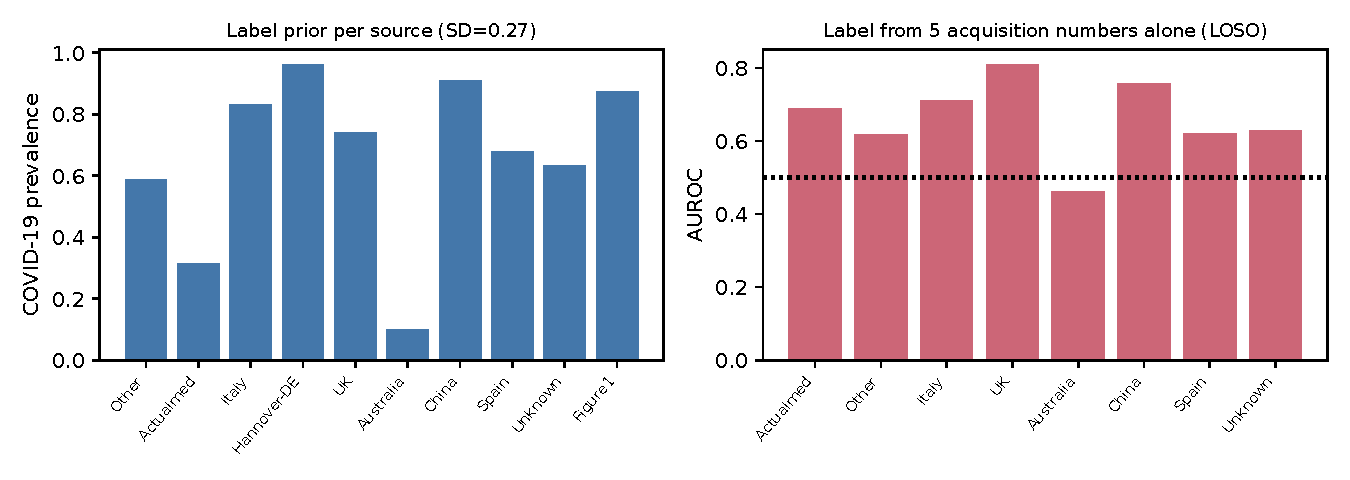
\includegraphics[width=\linewidth]{figures/fig_diagnostics.pdf}
\caption{Left: COVID-19 prevalence per source. Right: AUROC for predicting the diagnosis on a held-out site from five acquisition statistics alone (logistic regression, trained on the other sites).}\label{fig:diag}
\end{figure}
Model predictions co-vary with the same signal: within-class shortcut reliance is $\relErm$ for \erm{} and between $\relSiteProfileAug$ and $\relSidlFull$ for the other methods (Table~\ref{tab:reliance}); the methods designed to lower it (site-profile augmentation, PAI) lower it only slightly ($\relSiteProfileAug$ and $\relProfileAdversaryPai$ versus $\relErm$) and the two methods with a class-conditional adversary and prior reweighting have the \emph{highest} values ($\relSidlCc$, $\relSidlFull$).
\begin{table}[t]\centering\small
\begin{tabular}{lccc}
\toprule
Method & Dev.\ folds & Conf.\ folds & All 8 \\
\midrule
ERM & 0.456 & 0.419 & 0.438 \\
GroupDRO & 0.470 & 0.377 & 0.423 \\
DANN & 0.400 & 0.431 & 0.415 \\
Generic aug. & 0.457 & 0.366 & 0.411 \\
Site-profile aug. & 0.401 & 0.390 & 0.396 \\
Profile adversary (PAI) & 0.406 & 0.391 & 0.398 \\
SIDL-cc & 0.436 & 0.511 & 0.473 \\
SIDL-phys & 0.415 & 0.430 & 0.422 \\
SIDL-full & 0.500 & 0.528 & 0.514 \\
\bottomrule
\end{tabular}
\caption{Shortcut reliance (mean within-class Spearman correlation of held-out $P(\text{COVID-19})$ with a profile-only score), averaged over held-out sites and seeds.}\label{tab:reliance}
\end{table}

\subsection{No invariance method significantly beats \erm{}}\label{sec:task}
Table~\ref{tab:main} and Figure~\ref{fig:methods} summarize eight held-out sites. \erm{} reaches AUROC $\TErmAurocDev$ on the development folds and $\TErmAurocConf$ on the confirmation folds. The paired differences against \erm{} are small and every interval includes zero: GroupDRO $+\TGroupdroDiffVsErm$ [$\TGroupdroLo$, $\TGroupdroHi$], the site-profile augmentation plus unconditional adversary variant (SIDL-phys) $+\TSidlPhysDiffVsErm$ [$\TSidlPhysLo$, $\TSidlPhysHi$], generic augmentation $\TGenericAugDiffVsErm$, PAI $\TProfileAdversaryPaiDiffVsErm$, DANN $\TDannDiffVsErm$, site-profile augmentation alone $\TSiteProfileAugDiffVsErm$, SIDL-cc $\TSidlCcDiffVsErm$ and SIDL-full $\TSidlFullDiffVsErm$ [$\TSidlFullLo$, $\TSidlFullHi$]. The upper ends of the intervals exclude gains larger than about $0.055$ AUROC for every method. The ordering of methods is not stable across fold sets (Spearman correlation of method means between development and confirmation folds: $\rankCorrDevConf$): site-profile augmentation looked tied with \erm{} on the development folds ($\TSiteProfileAugAurocDev$ versus $\TErmAurocDev$) and fell below it on the confirmation folds ($\TSiteProfileAugAurocConf$ versus $\TErmAurocConf$), while SIDL-phys moved in the opposite direction.
\begin{table}[t]\centering\scriptsize
\resizebox{\linewidth}{!}{\begin{tabular}{lccccccc}
\toprule
Method & AUROC dev & AUROC conf. & AUROC all & Worst fold & $\Delta$ vs ERM [95\% CI] & Bal.\ acc. & ECE \\
\midrule
ERM & 0.758 & 0.707 & 0.733 & 0.565 & -- & 0.634 & 0.157 \\
GroupDRO & 0.761 & 0.735 & 0.748 & 0.657 & +0.015 [-0.015, +0.055] & 0.689 & 0.144 \\
DANN & 0.752 & 0.702 & 0.727 & 0.645 & -0.006 [-0.049, +0.035] & 0.599 & 0.166 \\
Generic aug. & 0.748 & 0.716 & 0.732 & 0.619 & -0.001 [-0.029, +0.032] & 0.663 & 0.150 \\
Site-profile aug. & 0.757 & 0.694 & 0.726 & 0.641 & -0.007 [-0.060, +0.038] & 0.618 & 0.174 \\
Profile adversary (PAI) & 0.753 & 0.708 & 0.730 & 0.551 & -0.002 [-0.020, +0.014] & 0.615 & 0.154 \\
SIDL-cc & 0.722 & 0.699 & 0.711 & 0.635 & -0.022 [-0.069, +0.030] & 0.612 & 0.178 \\
SIDL-phys & 0.756 & 0.732 & 0.744 & 0.650 & +0.011 [-0.016, +0.050] & 0.656 & 0.192 \\
SIDL-full & 0.738 & 0.665 & 0.701 & 0.415 & -0.031 [-0.085, +0.016] & 0.590 & 0.175 \\
\bottomrule
\end{tabular}}
\caption{Leave-one-site-out task metrics (mean over held-out sites of the two-seed mean). $\Delta$ is the paired AUROC difference to \erm{} over all eight sites with the hierarchical bootstrap $95\%$ interval. ``Worst fold'' is the lowest per-site AUROC (for \erm{} this is Australia, which has $6$ positive images). Balanced accuracy and ECE use the argmax decision.}\label{tab:main}
\end{table}
\begin{figure}[t]\centering
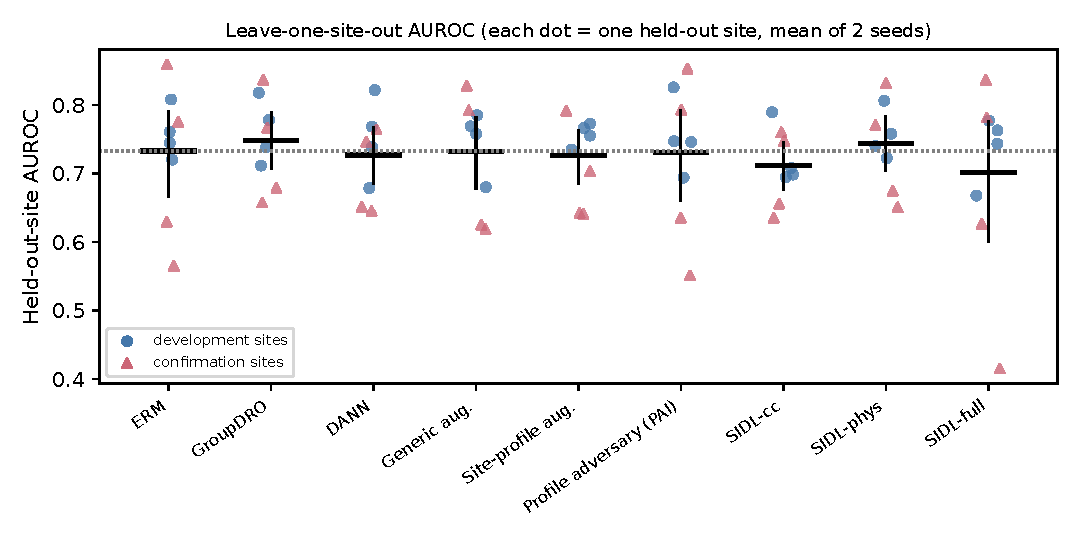
\includegraphics[width=0.92\linewidth]{figures/fig_methods.pdf}
\caption{Held-out-site AUROC for each method (dots: sites; black bar and line: mean and bootstrap interval over sites).}\label{fig:methods}
\end{figure}
Two caveats apply. First, GroupDRO has higher balanced accuracy ($\TGroupdroBalAcc$ versus $\TErmBalAcc$) and a higher worst-site AUROC ($\TGroupdroWorstFold$ versus $\TErmWorstFold$), but the worst site for \erm{} has only $6$ positives, PAI does not share the gain, and balanced accuracy at the argmax threshold depends on the operating point that group reweighting shifts; we treat these as exploratory. Second, the equivalence we report is for a small convolutional network trained from scratch at $64\times64$; we do not know whether it holds for large pretrained models.

\paragraph{Strong augmentation hurts.} In our first iteration, full-batch full-strength augmentation lowered development-fold AUROC by up to $0.083$ (generic augmentation: $0.675$ against $0.758$ for \erm{}). Making augmentation per-sample and milder (probability $0.3$, strength $0.5$) removed the drop ($0.748$), confirming that the earlier loss came from over-strong transformation, but no setting improved on \erm{}.

\subsection{Controlled label-shift experiments}\label{sec:synth}
On the semi-synthetic benchmark, with identical image content and known acquisition transforms, we swept the prior spread across virtual sites (Table~\ref{tab:synthls}, Figure~\ref{fig:synth}). At the largest spread ($0.4$), the paired differences to \erm{} are: DANN $\synthDiffDann$ [$\synthDiffDannLo$, $\synthDiffDannHi$], cDANN $\synthDiffCdann$ [$\synthDiffCdannLo$, $\synthDiffCdannHi$], cDANN with prior reweighting $\synthDiffCdannP$ [$\synthDiffCdannPLo$, $\synthDiffCdannPHi$] and prior reweighting alone $\synthDiffErmP$ [$\synthDiffErmPLo$, $\synthDiffErmPHi$]. The ordering at high label shift (cDANN with reweighting above cDANN above DANN) matches the theoretical expectation that unconditional alignment is the most harmful, but all adversaries are below \erm{}, and they already lose $0.02$ to $0.06$ AUROC at spread zero when the adversary weight is $0.5$. Shrinking the adversary weight brings it toward \erm{} (Table~\ref{tab:synthadv}) but never above it; the sign of the advantage of cDANN with reweighting over DANN flips across weights, so with six units per cell we cannot support a claim that the class-conditional adversary helps.
\begin{table}[t]\centering\small
\begin{tabular}{lccccc c}
\toprule
Prior spread & ERM & ERM+prior & DANN & cDANN & cDANN+prior & Units \\
\midrule
0.00 & 0.732 & 0.735 & 0.672 & 0.682 & 0.712 & 6 \\
0.25 & 0.721 & 0.725 & 0.681 & 0.685 & 0.681 & 6 \\
0.40 & 0.703 & 0.703 & 0.611 & 0.626 & 0.656 & 6 \\
\bottomrule
\end{tabular}
\caption{Semi-synthetic label-shift sweep: held-out AUROC (mean over virtual sites $V0,V2,V4$ and two seeds; adversary weight $0.5$; $6$ units per cell).}\label{tab:synthls}
\end{table}
\begin{table}[t]\centering\small
\begin{tabular}{llcccc}
\toprule
Method & Spread & $\lambda{=}0.02$ & $\lambda{=}0.1$ & $\lambda{=}0.5$ & ERM \\
\midrule
DANN & 0.0 & 0.719 & 0.694 & 0.694 & 0.720 \\
cDANN+prior & 0.0 & 0.721 & 0.720 & 0.688 & 0.720 \\
DANN & 0.4 & 0.736 & 0.743 & 0.602 & 0.740 \\
cDANN+prior & 0.4 & 0.756 & 0.743 & 0.730 & 0.740 \\
\bottomrule
\end{tabular}
\caption{Adversary-weight sweep on the semi-synthetic benchmark (held-out AUROC, $6$ units per cell, no augmentation).}\label{tab:synthadv}
\end{table}
\begin{figure}[t]\centering
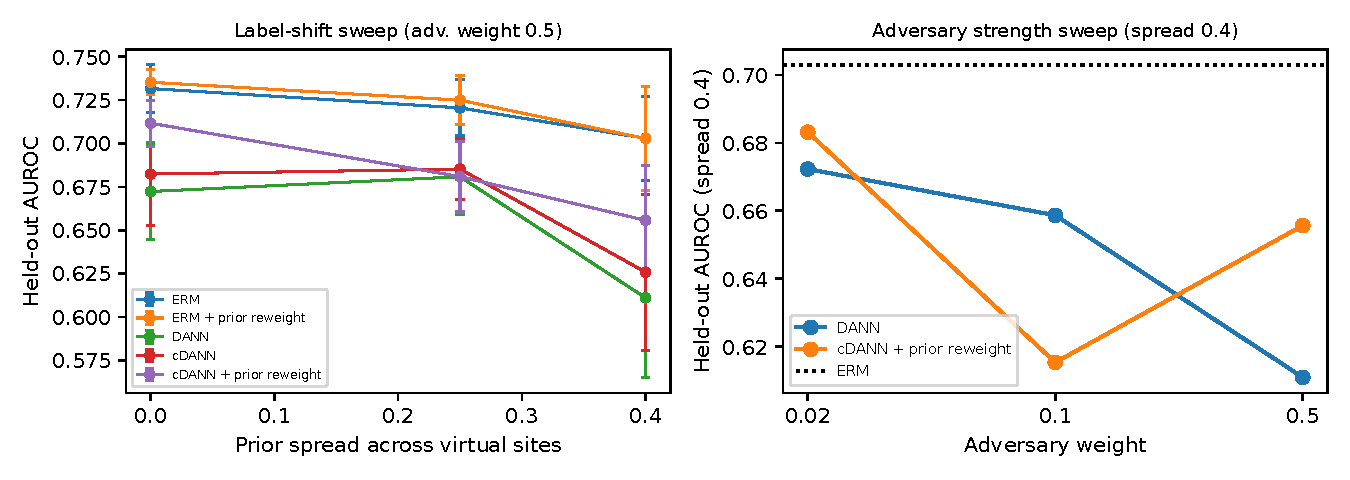
\includegraphics[width=\linewidth]{figures/fig_synth.pdf}
\caption{Semi-synthetic benchmark. Left: held-out AUROC as the label-prior spread across virtual sites grows (bars: standard error over $6$ units). Right: AUROC as the adversary weight shrinks, at spread $0.4$.}\label{fig:synth}
\end{figure}

\subsection{Calibrating prediction sets for unseen sites}\label{sec:conf}
Table~\ref{tab:conf} and Figure~\ref{fig:conf} report conformal results for the \erm{} model on all eight held-out sites at $\alpha=0.1$. Conformal sets calibrated on the validation split of seen source sites under-cover: mean coverage is $\CPooledCovMean$ (pooled) and $\CSiteBalancedCovMean$ (site-balanced) against the $0.90$ target, the lowest site coverage is about $\CPooledCovMin$, and $\CPooledNUnder$ of $\CPooledN$ sites are more than five points short. This pattern appears in both fold sets (development: $0.829$; confirmation: $0.843$ for pooled). Worst-site calibration restores mean coverage ($\CWorstSiteCovMean$) but still leaves two sites short (lowest $\CWorstSiteCovMin$, on the confirmation site ``Other''). The leave-site-out CV+ rule has mean coverage $\CLsoCvplusCovMean$, lowest site coverage $\CLsoCvplusCovMin$ and no site more than five points short, at mean set size $\CLsoCvplusSize$ against $\CPooledSize$ for pooled calibration. It over-covers on most sites; LSO-split, which applies the pooled leave-site-out quantile to the single deployed model, is nearer the target on average ($\CLsoSplitCovMean$) but has a site at $\CLsoSplitCovMin$.
\begin{table}[t]\centering\scriptsize
\resizebox{\linewidth}{!}{\begin{tabular}{lccccccc}
\toprule
Calibration & Cov. & Min cov. & Sites $<$0.85 & Size & Cov.\ calib.\ err. & Frac.\ under & Size@90\% \\
\midrule
Pooled (seen-site val.) & 0.836 & 0.743 & 4/8 & 1.39 & 0.048 & 0.389 & 1.58 \\
Site-balanced (seen-site val.) & 0.840 & 0.746 & 4/8 & 1.38 & 0.053 & 0.472 & 1.60 \\
Worst-site (seen-site val.) & 0.904 & 0.751 & 2/8 & 1.60 & 0.009 & 0.236 & 1.58 \\
LSO-split & 0.905 & 0.732 & 1/8 & 1.59 & 0.011 & 0.208 & 1.57 \\
LSO-split, balanced & 0.886 & 0.711 & 1/8 & 1.54 & 0.009 & 0.236 & 1.58 \\
LSO-worst-site & 0.960 & 0.832 & 1/8 & 1.81 & 0.083 & 0.028 & 1.59 \\
LSO-CV+ & 0.942 & 0.867 & 0/8 & 1.75 & 0.041 & 0.069 & 1.60 \\
LSO-CV+, balanced & 0.926 & 0.792 & 1/8 & 1.69 & 0.020 & 0.153 & 1.60 \\
\bottomrule
\end{tabular}}
\caption{Conformal prediction on the held-out sites for the \erm{} model ($\alpha=0.1$, target coverage $0.90$; eight sites, two seeds). Cov.\ and Size are means over sites at $\alpha=0.1$; ``Folds $<0.85$'' counts sites more than five points below target; the last three columns are computed over the $\alpha$ grid (Section~\ref{sec:confmethods}). Rows 1--3 calibrate on seen-site validation data; rows 4--8 use leave-site-out scores.}\label{tab:conf}
\end{table}
\begin{figure}[t]\centering
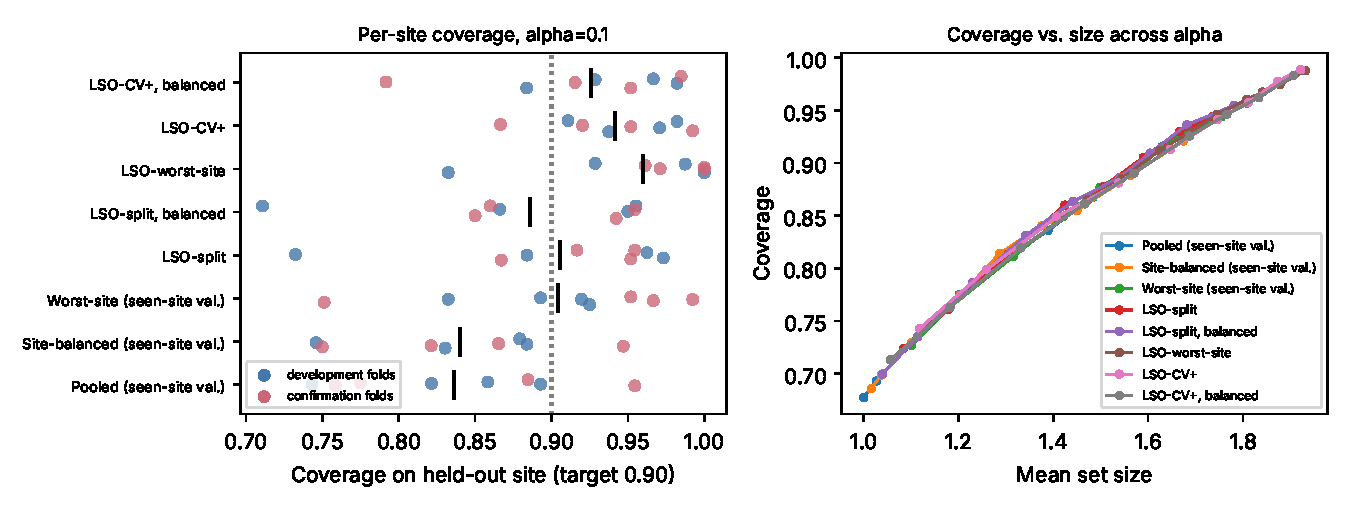
\includegraphics[width=\linewidth]{figures/fig_conformal.pdf}
\caption{Left: coverage on each held-out site at $\alpha=0.1$ (bar: mean). Right: coverage versus set size over the $\alpha$ grid, averaged over sites; all calibrations lie on nearly one curve.}\label{fig:conf}
\end{figure}
\paragraph{Calibrations differ in operating point, not efficiency.} Interpolated at $90\%$ coverage the mean set size is between $\CLsoSplitSizeAtCov$ and $\CSiteBalancedSizeAtCov$ for \emph{every} calibration, including pooled ($\CPooledSizeAtCov$) and LSO-CV+ ($\CLsoCvplusSizeAtCov$); the development folds had suggested that LSO-CV+ was about $4\%$ smaller at matched coverage, which the confirmation folds did not reproduce. The benefit of leave-site-out calibration is therefore \emph{safety} (it lands at a conservative point on the same curve without being told the target site's shift) and not a smaller set. Whether a clinician prefers sets about $26\%$ larger to a mean coverage shortfall of about six points (up to sixteen at the worst site) is an application decision.

\paragraph{Negative results on conformal variants.} Two further variants did not help on the development folds and were dropped: weighting calibration scores by a density ratio of the label-free acquisition profile between source and target images (coverage $0.834$ against $0.829$ for pooled), and correcting for estimated label shift with an EM prior estimate~\cite{saerens2002adjusting} or a label-shift-weighted conformal rule~\cite{podkopaev2021distribution} (coverage $0.813$ with the EM prior and $0.845$ with the oracle prior, against $0.829$ for pooled; EM prior-estimation error $0.186$ and balanced accuracy got worse after adjustment). Covariate and calibration shift dominate over label shift on this data.

\subsection{Why seen-site calibration under-covers: validation optimism}\label{sec:optim}
For each held-out site we compared three quantities for the \erm{} model: the AUROC on the validation split of seen sites, the leave-site-out estimate (mean AUROC of the inner models on the sites they did not see), and the actual held-out AUROC (Figure~\ref{fig:optim}). Over $\ONUnits$ fold--seed units, seen-site validation overstates held-out AUROC by $\OMeanSignedSeen$ on average (mean absolute error $\OMaeSeen$), whereas the leave-site-out estimate is nearly unbiased ($\OMeanSignedLso$; mean absolute error $\OMaeLso$). Neither estimator ranks sites (Spearman correlation with the actual AUROC across the eight sites: $\ORhoSeen$ for seen-site validation and $\ORhoLso$ for leave-site-out), because actual AUROC ranges from $0.56$ to $0.86$ while the leave-site-out estimate stays between $0.72$ and $0.75$: the estimate describes the typical unseen site, not a particular one. The per-site optimism gap and the pooled-conformal coverage are rank-correlated in the expected direction ($\ORhoGapCov$ across eight sites), which is consistent with optimism being the mechanism for under-coverage but is not significant at this sample size. A site-bagged ensemble of the inner models, a free by-product, has held-out AUROC $\ensAurocEns$ against $\ensAurocFull$ for the single full model ($\ensDAuroc$ [$\ensDAurocLo$, $\ensDAurocHi$]; better on $\ensFoldsBetter$ of 8 sites; ECE change $\ensDEce$), i.e.\ no significant gain.
\begin{figure}[t]\centering
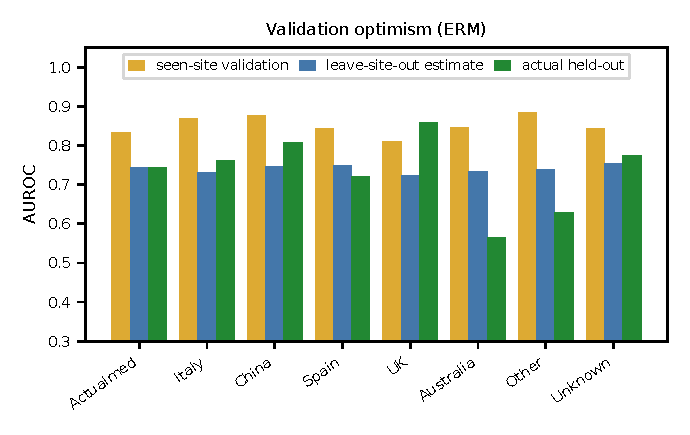
\includegraphics[width=0.85\linewidth]{figures/fig_optimism.pdf}
\caption{AUROC of the \erm{} model estimated on seen-site validation data, estimated by leave-site-out models, and actually obtained on the held-out site (mean of two seeds).}\label{fig:optim}
\end{figure}

\subsection{Simulated acquisition shift does not reproduce real under-coverage}\label{sec:realism}
On the semi-synthetic benchmark with known acquisition transforms of three severities, seen-site calibration is already well calibrated (Table~\ref{tab:synthconf}): pooled coverage is $0.896$--$0.922$ against the $0.90$ target, in contrast to $\CPooledCovMean$ on real sites. The leave-site-out variants are not better, and LSO-split under-covers at the highest severity ($0.834$, lowest site $0.688$). The real under-coverage therefore comes from inter-site differences beyond the acquisition statistics we simulate (patient population, case selection, labeling and image provenance). A calibration method validated only on simulated acquisition shift would have looked adequate here.
\begin{table}[t]\centering\scriptsize
\resizebox{\linewidth}{!}{\begin{tabular}{lcccccc}
\toprule
Severity & Pooled & Site-bal. & Worst-site & LSO-split & LSO-CV+ & LSO-worst \\
\midrule
0.5 & 0.896 (0.875) / 1.37 & 0.892 (0.878) / 1.36 & 0.909 (0.866) / 1.44 & 0.933 (0.931) / 1.55 & 0.928 (0.894) / 1.54 & 0.964 (0.956) / 1.70 \\
1.0 & 0.922 (0.878) / 1.58 & 0.910 (0.878) / 1.54 & 0.912 (0.828) / 1.55 & 0.918 (0.906) / 1.54 & 0.931 (0.891) / 1.55 & 0.965 (0.950) / 1.72 \\
1.5 & 0.921 (0.916) / 1.65 & 0.908 (0.878) / 1.61 & 0.920 (0.906) / 1.66 & 0.834 (0.688) / 1.43 & 0.931 (0.859) / 1.66 & 0.960 (0.891) / 1.79 \\
\bottomrule
\end{tabular}}
\caption{Semi-synthetic benchmark, conformal coverage (lowest virtual-site coverage) / mean set size at $\alpha=0.1$, three acquisition-severity levels (prior spread $0.25$; $3$ held-out virtual sites $\times$ $2$ seeds).}\label{tab:synthconf}
\end{table}

\section{Discussion and Limitations}\label{sec:disc}
\paragraph{What the evidence supports.} (a) On this benchmark, adding augmentation, site adversaries, profile adversaries, CORAL or GroupDRO to a small CNN did not significantly improve held-out-site AUROC; we can rule out gains larger than about $0.055$. (b) Acquisition statistics alone leak the diagnosis across sites, and model scores correlate with them within class, but the methods that reduce this correlation did not improve accuracy, so we cannot say that the shortcut is the cause of the accuracy loss. (c) Seen-site validation is optimistic about unseen sites and standard conformal sets under-cover them; leave-site-out calibration avoids severe under-coverage without a smaller set. (d) Simulated acquisition shift is a poor proxy for inter-hospital shift in this dataset.

\paragraph{Why invariance may not help here (untested).} The dataset is tiny ($\datasetTotal$ images, held-out sites of $52$--$207$ images), the encoder is trained from scratch at $64\times64$, the diagnosis-correlated acquisition signal seems to be mostly within-site, and the sites themselves differ in case selection. Adversarial objectives add optimization noise that a small network may not afford: even with exactly known acquisition shift, adversaries lost AUROC at every weight we tried. These are hypotheses, not findings.

\paragraph{Limitations.} \emph{Scope:} one modality (chest radiographs) and one task, although the title speaks of medical image diagnosis in general; our environment could not reach the credentialed or large datasets (CheXpert, MIMIC-CXR, Camelyon17-WILDS, fundus and MRI collections) and had no GPU or pretrained weights. We used no private data. \emph{Data quality:} the collection is retrospective, assembled from publications and case reports, with positive and negative examples from different sources; COVID-19 labels here reflect collection practice, so absolute AUROC is not clinically meaningful. ``Other'' and ``Unknown'' are mixtures of institutions. \emph{Statistics:} eight held-out sites, two seeds per cell, tiny test sets for some sites, many comparisons and no multiplicity correction; our intervals are wide and ``no significant difference'' is not evidence of equivalence for effects below roughly $0.03$ AUROC. The development/confirmation split was assigned by us and not randomized. Hyperparameters were tuned on development folds with modest budgets, so a better-tuned variant could still help. \emph{Conformal:} none of the leave-site-out rules has a finite-sample guarantee under site shift; the observed coverage depends on the particular set of sites. Coverage is marginal over test images in a site, not conditional on class or patient. \emph{Profile estimators} are proxies and our augmentation is not a scanner simulator.

\paragraph{Implications.} For multi-site medical imaging with small data, our results argue for (i) reporting leave-site-out performance with site-level uncertainty rather than pooled validation numbers, (ii) treating a strong \erm{} baseline with leave-site-out-calibrated sets as the reference any invariance method must beat, and (iii) validating calibration methods on real multi-site data, not only on simulated acquisition shift. A claim that invariance helps would require larger data, stronger encoders and more sites than we could access.

\section{Conclusion}
A scanner- and institution-invariant training recipe built from class-conditional alignment and site-profile augmentation did not improve held-out-site accuracy over empirical risk minimization on an open multi-source chest-radiograph benchmark, under a protocol that froze configurations before the confirmation sites were run. The durable results are a label-free leak diagnostic, a quantified gap between seen-site validation and leave-site-out performance, the finding that standard conformal sets under-cover unseen sites and that leave-site-out CV+ calibration avoids severe under-coverage by trading set size, and the observation that simulated acquisition shift does not reproduce the real effect.

\paragraph{Reproducibility.} All code, frozen configurations, per-run result files and the script \texttt{scripts/\allowbreak final\_report.py}, which regenerates every table, figure and headline number in this paper from the raw run files, are in the accompanying repository (side analyses quoted in running text, such as the conformal variants on development folds, the label-shift correction and the leak-removal check, come from the scripts named in the iteration log); the benchmark is rebuilt from the three public collections by \texttt{scripts/\allowbreak build\_covid\_cxr.py}. An iteration log (\texttt{experiments/\allowbreak ITERATIONS.md}) records every experiment, including those that failed, and the confirmation folds were not inspected before the single frozen run. An early iteration-1 run had started on two confirmation sites; those partial outputs were not used in any analysis or decision and are excluded.

\paragraph{AI assistance and ethics.} The code, experiments and a first draft of this paper were produced with an AI coding assistant (Claude), under human direction; all reported numbers were generated by the released code, and the authors are responsible for the content. The study uses only public, de-identified images; no patient-level clinical decision is made or implied.

\bibliographystyle{plainnat}
\bibliography{refs}

\appendix
\section{Per-site AUROC}
\begin{table}[H]\centering\scriptsize
\resizebox{\linewidth}{!}{\begin{tabular}{lcccccccc}
\toprule
Method & Actualmed$^{d}$ & Italy$^{d}$ & China$^{d}$ & Spain$^{d}$ & UK$^{c}$ & Australia$^{c}$ & Other$^{c}$ & Unknown$^{c}$ \\
\midrule
ERM & 0.745 & 0.761 & 0.808 & 0.720 & 0.859 & 0.565 & 0.629 & 0.775 \\
GroupDRO & 0.778 & 0.738 & 0.818 & 0.711 & 0.837 & 0.679 & 0.657 & 0.766 \\
DANN & 0.768 & 0.739 & 0.822 & 0.678 & 0.746 & 0.651 & 0.645 & 0.764 \\
Generic aug. & 0.785 & 0.757 & 0.769 & 0.680 & 0.828 & 0.625 & 0.619 & 0.792 \\
Site-profile aug. & 0.755 & 0.766 & 0.773 & 0.735 & 0.703 & 0.642 & 0.641 & 0.791 \\
Profile adversary (PAI) & 0.747 & 0.746 & 0.825 & 0.694 & 0.853 & 0.551 & 0.635 & 0.793 \\
SIDL-cc & 0.698 & 0.789 & 0.708 & 0.694 & 0.747 & 0.656 & 0.635 & 0.760 \\
SIDL-phys & 0.740 & 0.758 & 0.806 & 0.722 & 0.831 & 0.674 & 0.650 & 0.770 \\
SIDL-full & 0.763 & 0.777 & 0.743 & 0.667 & 0.782 & 0.415 & 0.626 & 0.837 \\
\bottomrule
\end{tabular}}
\caption{Held-out AUROC per site (mean of two seeds); superscript d = development fold, c = confirmation fold.}\label{tab:perfold}
\end{table}
\section{Iteration summary}
The development followed ten documented iterations (full details in \texttt{experiments/\allowbreak ITERATIONS.md}): (0)~label-free diagnostics; (1)~baselines and first SIDL variants, where strong full-batch augmentation hurt; (2)~per-sample augmentation strength, which removed the drop but gave no gain; (3)~semi-synthetic label-shift sweep; (4)~adversary-strength sweep; (5)~profile-adversarial invariance and test-time label-shift handling, both negative; (6)~leave-site-out conformal and optimism analysis on development folds; (7)~leave-site-out conformal on semi-synthetic shift, which did not reproduce real under-coverage; (8)~mild-setting SIDL variants and configuration freezing; (9)~frozen confirmation run on the untouched sites; (10)~consolidation with hierarchical statistics, the ensemble check and the generated report.
\end{document}
